
\documentclass{article}
\usepackage[utf8]{inputenc}
\usepackage[T1]{fontenc}
\usepackage{graphicx}
\usepackage{geometry}


\title{TP1 Simulation de Système }
\author{Terenui Rouby et Karim Mouaddel}
\geometry{hmargin=2.5cm,vmargin=1.5cm}

\begin{document}

\maketitle
\pagenumbering{gobble}
\thispagestyle{empty}

\newpage
\pagenumbering{gobble}
\tableofcontents

\newpage
\pagenumbering{gobble}
\section{Partie 1}
\subsection{Dealer}
\subsection{Mélange du deck}
Afin d'effectuer le mélange du jeu de carte on utilise la méthode \textit{shuffle()} qui est inclut dans la classe dealer. On s'est inspiré pour implémenter cette méthode d'une méthode de mélange de jeu de cartes que l'on a trouvé sur internet. Pour effectuer ce mélange nous avons utilisé la méthode Random provenant de la bibliothèque java.util qui est un générateur de nombre pseudo aléatoire en java.
\subsection{Résultat}
\vspace{0.5cm}
	\begin{flushleft}
{\renewcommand{\arraystretch}{2} %donne la distance entre les lignes%
{\setlength{\tabcolsep}{1.5cm} %donne la distance entre les collones%
	\begin{tabular}{|c|c|}
			\hline
			Numéro du jeu & Pourcentage de victoire\\ \hline
			1 & 7,7484 \\ \hline
			2 & 1,9175 \\ \hline
			3 & 47,1514 \\ \hline
			4 & 98,7167 \\ \hline
			5 & 5,1754 \\
				\hline

		\end{tabular}}}

	\end{flushleft}

\subsection{Pertinence des résultat}
\subsubsection{Game 1}
\subsubsection{Game 2}
\subsubsection{Game 3}
\subsubsection{Game 4}
\subsubsection{Game 5}


\clearpage

\newpage
\section{Partie 2}
\begin{figure}[htbp]
	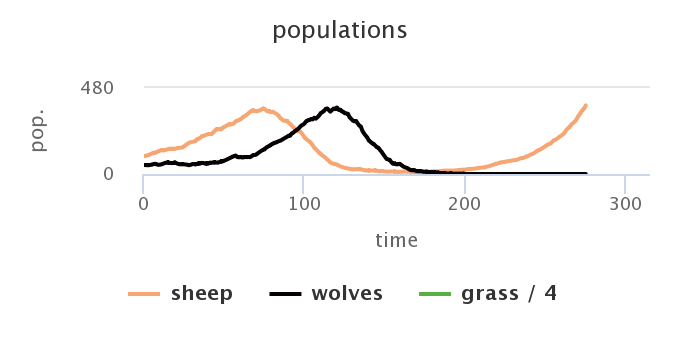
\includegraphics[width=1.0\textwidth]{chart.png}
		\caption{Graphique d'une simulation Prédateur Proie normale}
	\label{fig:chart}
\end{figure}

Quand le paramètre grass regrowth time est mis à 10 les moutons se déplacent très peu. De ce fait lorsque la population de mouton diminue les loups dépensent plus d’énergie pour les atteindre. Arrivé à un certain point la population de loup disparait par manque de nourriture(plus d’energie) car ils ne peuvent pas atteindre les moutons isolés(si il en reste).

\end{document}